\begin{exercice} %1
    Placer les points donnés sur chaque droite.
    \begin{enumerate}
        \item $A(\num{11.5})$; \hfill $B(\num{8.5})$; \hfill $C(\num{9.7})$; \hfill $D(\num{8.1})$;

        \medskip
        \raisebox{-0.5\totalheight}[0.5\totalheight]{\raisebox{\depth}{
        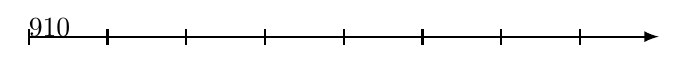
\begin{tikzpicture}[scale=1]            
            % Axe
            \draw[thick,>=latex,->](0,0)--+(8,0);
            \foreach \x in {0,...,7} \draw[thick] (\x,-.1) -- (\x,0.1);
            \coordinate (O) at (2,0);
            \coordinate (I) at (4,0);
            \draw[thick] (2,-.1) -- (2,0.1);
            \draw[thick] (4,-.1) -- (4,0.1);
            \tkzLabelPoint[below,yshift=-3](O){$9$};
            \tkzLabelPoint[below,yshift=-3](I){$10$};
            \tkzLabelPoint[above](O){\phantom{$O$}};
            \papierMillimetre
        \end{tikzpicture}
        }}
        \medskip
        \item $E(\num{0.2})$; \hfill $F(\num{0.55})$; \hfill $G(\num{0.73})$; \hfill $H(\num{0.40})$;
        
        \medskip
        \raisebox{-0.5\totalheight}[0.5\totalheight]{\raisebox{\depth}{
        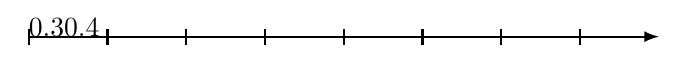
\begin{tikzpicture}[scale=1]            
            % Axe
            \draw[thick,>=latex,->](0,0)--+(8,0);
            \foreach \x in {0,...,7} \draw[thick] (\x,-.1) -- (\x,0.1);
            \coordinate (O) at (2,0);
            \coordinate (I) at (3,0);
            \draw[thick] (2,-.1) -- (2,0.1);
            \draw[thick] (3,-.1) -- (3,0.1);
            \tkzLabelPoint[below,yshift=-3](O){$\num{0.3}$};
            \tkzLabelPoint[below,yshift=-3](I){$\num{0.4}$};
            \tkzLabelPoint[above](O){\phantom{$O$}};
            \papierMillimetre
        \end{tikzpicture}
        }}
        \medskip
        \item $J(\num{5.33})$; \hfill $K(\num{5.28})$; \hfill $L(\num{5.315})$; \hfill $M(\num{5.304})$;
        
        \medskip
        \raisebox{-0.5\totalheight}[0.5\totalheight]{\raisebox{\depth}{
        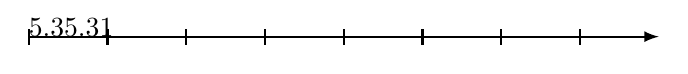
\begin{tikzpicture}[scale=1]            
            % Axe
            \draw[thick,>=latex,->](0,0)--+(8,0);
            \foreach \x in {0,...,7} \draw[thick] (\x,-.1) -- (\x,0.1);
            \coordinate (O) at (3,0);
            \coordinate (I) at (4,0);
            \draw[thick] (3,-.1) -- (3,0.1);
            \draw[thick] (4,-.1) -- (4,0.1);
            \tkzLabelPoint[below,yshift=-3](O){$\num{5.3}$};
            \tkzLabelPoint[below,yshift=-3](I){$\num{5.31}$};            
            \tkzLabelPoint[above](O){\phantom{$O$}};
            \papierMillimetre
        \end{tikzpicture}
        }}
    \end{enumerate}
 \end{exercice}
 
 \begin{corrige}
    Placer les points donnés sur chaque droite.

    \begin{enumerate}
        \item $A(\num{11.5})$; \hfill $B(\num{8.5})$; \hfill $C(\num{9.7})$; \hfill $D(\num{8.1})$;

        \medskip
        \raisebox{-0.5\totalheight}[0.5\totalheight]{\raisebox{\depth}{
        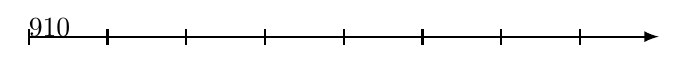
\begin{tikzpicture}[scale=1]            
            % Axe
            \draw[thick,>=latex,->](0,0)--+(8,0);
            \foreach \x in {0,...,7} \draw[thick] (\x,-.1) -- (\x,0.1);
            \coordinate (O) at (2,0);
            \coordinate (I) at (4,0);
            \draw[thick] (2,-.1) -- (2,0.1);
            \draw[thick] (4,-.1) -- (4,0.1);
            \tkzLabelPoint[below,yshift=-3](O){$9$};
            \tkzLabelPoint[below,yshift=-3](I){$10$};
            % Correction
            % Points supplémentaires
            \coordinate (A) at (7,0);
            \coordinate (B) at (1,0);
            \coordinate (C) at (3.4,0);
            \coordinate (D) at (0.2,0);
            \tkzDrawPoints[shape=cross out,size=3pt,color=red](A,B,C,D);
            \tkzLabelPoints[above,color=red](A,B,C,D);
            \papierMillimetre
        \end{tikzpicture}
        }}
        \medskip
        \item $E(\num{0.2})$; \hfill $F(\num{0.55})$; \hfill $G(\num{0.73})$; \hfill $H(\num{0.40})$;
        
        \medskip
        \raisebox{-0.5\totalheight}[0.5\totalheight]{\raisebox{\depth}{
        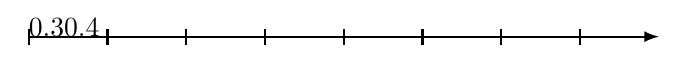
\begin{tikzpicture}[scale=1]            
            % Axe
            \draw[thick,>=latex,->](0,0)--+(8,0);
            \foreach \x in {0,...,7} \draw[thick] (\x,-.1) -- (\x,0.1);
            \coordinate (O) at (2,0);
            \coordinate (I) at (3,0);
            \draw[thick] (2,-.1) -- (2,0.1);
            \draw[thick] (3,-.1) -- (3,0.1);
            \tkzLabelPoint[below,yshift=-3](O){$\num{0.3}$};
            \tkzLabelPoint[below,yshift=-3](I){$\num{0.4}$};
            % Correction
            % Points supplémentaires
            \coordinate (E) at (1,0);
            \coordinate (F) at (5.5,0);
            \coordinate (G) at (7.3,0);
            \coordinate (H) at (3,0);
            \tkzDrawPoints[shape=cross out,size=3pt,color=red](E,F,G,H);
            \tkzLabelPoints[above,color=red](E,F,G,H);
            \papierMillimetre
        \end{tikzpicture}
        }}
        \medskip
        \item $J(\num{5.33})$; \hfill $K(\num{5.28})$; \hfill $L(\num{5.315})$; \hfill $M(\num{5.304})$;
        
        \medskip
        \raisebox{-0.5\totalheight}[0.5\totalheight]{\raisebox{\depth}{
        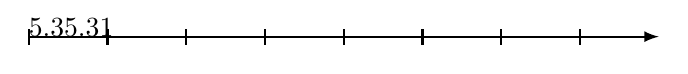
\begin{tikzpicture}[scale=1]            
            % Axe
            \draw[thick,>=latex,->](0,0)--+(8,0);
            \foreach \x in {0,...,7} \draw[thick] (\x,-.1) -- (\x,0.1);
            \coordinate (O) at (3,0);
            \coordinate (I) at (4,0);
            \draw[thick] (3,-.1) -- (3,0.1);
            \draw[thick] (4,-.1) -- (4,0.1);
            \tkzLabelPoint[below,yshift=-3](O){$\num{5.3}$};
            \tkzLabelPoint[below,yshift=-3](I){$\num{5.31}$};
            % Correction
            % Points supplémentaires
            \coordinate (J) at (6,0);
            \coordinate (K) at (1,0);
            \coordinate (L) at (4.5,0);
            \coordinate (M) at (3.4,0);
            \tkzDrawPoints[shape=cross out,size=3pt,color=red](J,K,L,M);
            \tkzLabelPoints[above,color=red](J,K,L,M);
            \papierMillimetre
        \end{tikzpicture}
        }}
    \end{enumerate}
 \end{corrige}
